\section{搭建Hadoop HA}
\subsection{简介}
上面配置的Hadoop尽管有了\lstinline{SecondaryNameNode}等机制来避免名称节点单点故障,但是
依然很不健壮,单点故障依然是存在的。Hadoop2中引入了HA(High Available)高可用机制,来确保Hadoop集群能够运行
24小时不宕机。需要搭配Zookeeper实现高可用。

\subsection{配置文件}
HA的配置相对比较复杂,主要需要修改的文件与配置分布式Hadoop时相同,可以参考第\ref{sec:hadoop_install}部分,重复部分不再赘述。
\lstinputlisting[style=myxml,title=core-site.xml]{docs/hadoop/hadoop/core-site.xml}
\begin{itemize}
	\item \lstinline{fs.defaultFS},HDFS对外暴露的服务端口。这里设置成了一个集群端口,而不是一个名称节点的端口。
			因为在HA中,一个集群中可能会有多个名称节点,但Active的只有一个,具体是哪个取决于Zookeeper。这里没有指定端口,
			使用的是默认的8020(新版本Hadoop的端口)。
	\item \lstinline{ha.zookeeper.quorum}指定了ZK集群有哪些机器。2181是ZK Client的默认端口,也可以在\lstinline{zoo.cfg}中配置。
	\item \lstinline{hadoop.proxyuser.zhangyu.hosts}该配置和下面的配置是为了解决Hive运行时权限验证的问题,这里设置为全部主机和用户组,即免去验证。
\end{itemize}
\lstinputlisting[style=myxml,title=hdfs-site.xml]{docs/hadoop/hadoop/ha.hdfs-site.xml}
\begin{itemize}
	\item \lstinline{dfs.nameservices},HDFS的名称服务,非常重要,而且要与\lstinline{core-site.xml}中的设置相对应。
	\item \lstinline{dfs.ha.namenodes.ldcluster},集群中的名称节点数。在当前名称节点宕机后,这些节点都有可能转换为Active状态。
	\item \lstinline{dfs.namenode.name.dir},保存名称节点元数据的目录。这里设置了很上面分布式不同的目录,方便切换。
	\item \lstinline{dfs.datanode.data.dir},同上。
	\item \lstinline{dfs.namenode.rpc-address.ldcluster.master},名称节点RPC通信的地址。设置默认的8020。注意要与\lstinline{nameservices}与\lstinline{namenodes}对应。
	\item \lstinline{dfs.namenode.rpc-address.ldcluster.slave1},同上。
	\item \lstinline{dfs.namenode.http-address.ldcluster.master},是查看HTTP服务也就是后面的Web界面的地址。原来是50070,新版本是9870。
	\item \lstinline{dfs.namenode.http-address.ldcluster.slave1},同上。
	\item \lstinline{dfs.namenode.shared.edits.dir},这里设置JournalNode的地址。HA是通过共享日志信息来查看是否有机器发生故障的。\lstinline{qjournal}是协议的名称,所有的机器都要加入进来,端口不用修改用默认。
	\item \lstinline{dfs.client.failover.proxy.provider.ldcluster},提供故障恢复的Java类,需要指定为:org.apache.hadoop.hdfs.server.
	namenode.ha.ConfiguredFailoverProxyProvider,不需要修改。
	\item \lstinline{dfs.ha.fencing.methods},故障后需要将原来的故障NameNode阻拦,采用\lstinline{sshfence}方式阻拦。
	\item \lstinline{dfs.ha.fencing.ssh.private-key-files},SSH私钥保存位置。
	\item \lstinline{dfs.ha.fencing.ssh.connect-timeout},SSH连接timeout时长,设置为30000。
	\item \lstinline{dfs.journalnode.edits.dir},保存JournalNode数据的目录,需要设置,且需要提前创建。
	\item \lstinline{dfs.ha.automatic-failover.enabled},设置开启自动故障恢复。
\end{itemize}
\lstinputlisting[style=myxml,title=yarn-site.xml]{docs/hadoop/hadoop/ha.yarn-site.xml}
\begin{itemize}
	\item \lstinline{yarn.resourcemanager.cluster-id},同\lstinline{hdfs-site.xml}中的\lstinline{nameservices}类似,为集群设置一个id,可自定义。
	\item \lstinline{yarn.resourcemanager.ha.rm-ids},资源管理器的id。这里设置为\lstinline{rm1},\lstinline{rm2},需要在后面明确指定主机地址。
	\item \lstinline{yarn.resourcemanager.hostname.rm1},指定\lstinline{rm1}为master机器。
	\item \lstinline{yarn.resourcemanager.hostname.rm2},同上指定\lstinline{rm2}。
	\item \lstinline{yarn.resourcemanager.webapp.address.rm1},通信地址。
	\item \lstinline{yarn.resourcemanager.webapp.address.rm2},同上。
	\item \lstinline{hadoop.zk.address},指定ZK集群地址。
	\item \lstinline{yarn.application.classpath},指定CLASSPATH。在执行MapReduce测试程序和Hive操作时,出现找不到主类的错误。可以在这里指定。
	\item \lstinline{yarn.log-aggregation-enable},为开启日志聚合功能,不涉及HA。
	\item \lstinline{yarn.log-aggregation.retain-seconds},日志保留的天数,这里是7天。
\end{itemize}
\lstinputlisting[style=myxml,title=mapred-site.xml]{docs/hadoop/hadoop/ha.mapred-site.xml}
\begin{itemize}
	\item \lstinline{mapreduce.application.classpath},设置MapReduce的CLASSPATH,还是为了解决前面的报错。
	\item \lstinline{mapreduce.jobhistory.address},JobHistory的地址。
	\item \lstinline{mapreduce.jobhistory.webapp.address},查看JobHistory的Web地址。
\end{itemize}

配置好之后,启动进程的顺序也很重要。
\begin{lstlisting}[style=mysh, title=启动步骤]
# 格式化ZK集群
hdfs zkfc -formatZK
# 格式化名称节点
hdfs namenode --format
# 将Master上格式化后名称节点目录下的内容
# 复制到Slave1对应配置的目录下面
# 不这样执行Slave1上的NameNode将无法启动
scp -r /data/name/* slave1:/data/name
# 启动HDFS,可以看到NameNode,DataNode,
# JournalNode,ZKFailoverController等节点的启动
start-dfs.sh
# 启动YARN
start-yarn.sh
# 可以看到ResourceManager和NodeManager在Master和Slave1上启动
jps
# 输出所有Java进程
\end{lstlisting}

\subsection{HDFS Shell操作}

关于HDFS的Shell命令行操作,比较简单,基本与常规的Linux Shell操作类似,只是
在前面加上\lstinline{hadoop fs}或\lstinline{hdfs dfs},个人常用后者。

如Linux \lstinline{ls}对应于\lstinline{hadoop fs -ls}或\lstinline{hdfs dfs -ls}。
类似还有\lstinline{hadoop fs -mkdir}或\lstinline{hdfs dfs -mkdir}。

上传文件为\lstinline{hdfs dfs -put}+ 目标的文件目录。
下载文件为\lstinline{hdfs dfs -get}+ 目标文件。

\label{subsec:hadoop_web}

\subsection{Hadoop Web UI}
可以通过http://master:9870 访问HDFS和查看整个集群信息概览。这里的master指的是名称节点的主机名。如果master挂了,可以使用其他的节点,如slave1访问。
这里也体现了HA的强大。

\begin{center}
	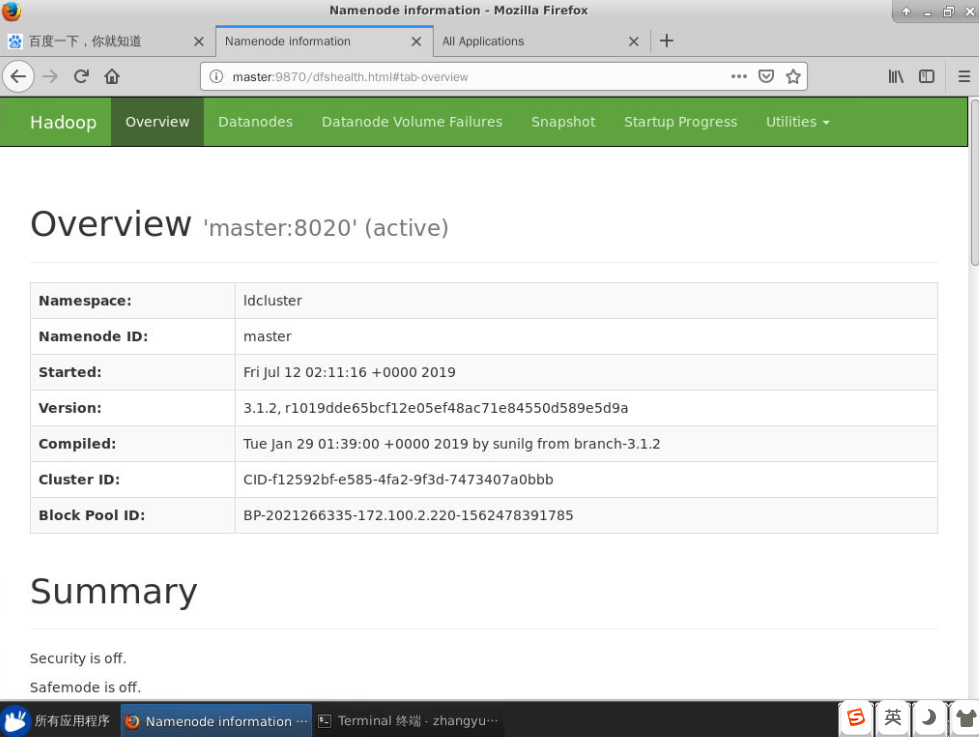
\includegraphics[width=\linewidth]{hadoop/hdfsweb1.png}
	
	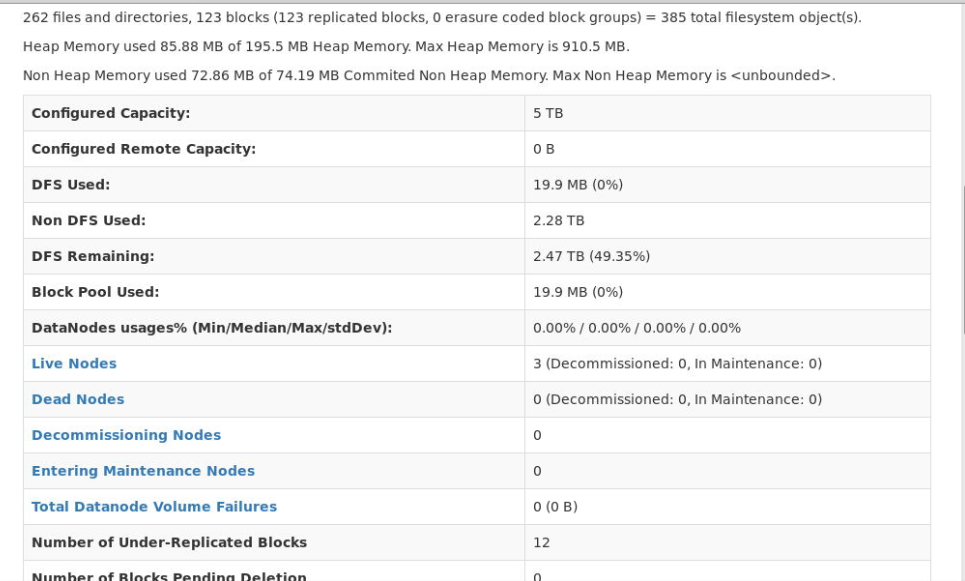
\includegraphics[width=\linewidth]{hadoop/hdfsweb2.png}

	在这里可以看到整个集群的概览信息,包括名称节点是否是活跃的,数据节点的活跃情况,日志节点信息

	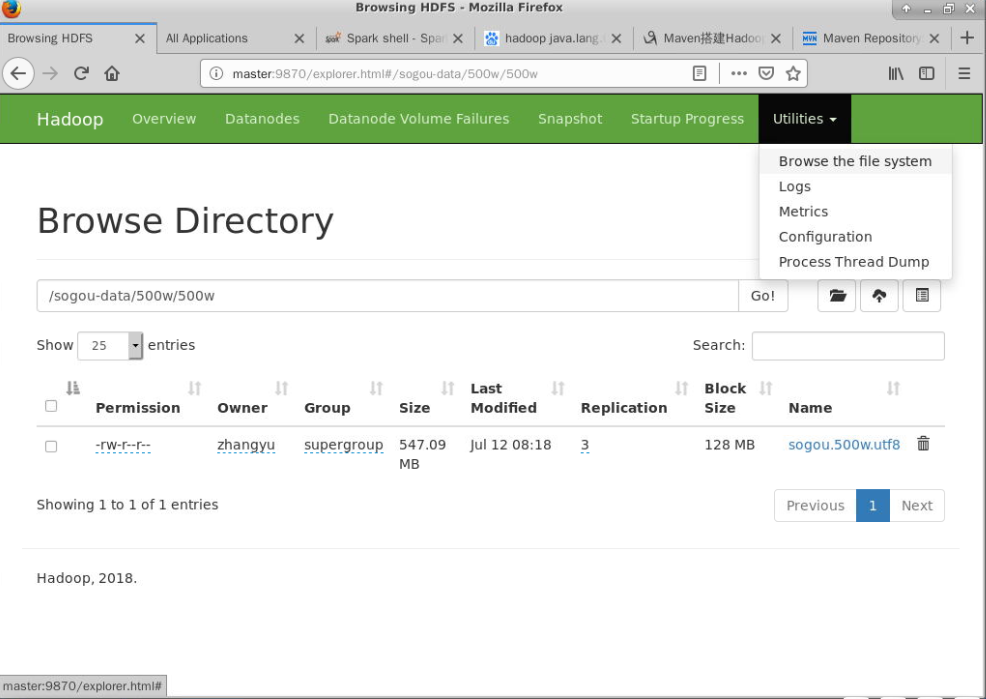
\includegraphics[width=\linewidth]{hadoop/filesys.png}
	
	浏览HDFS文件系统是非常有用的功能,还可以查看日志、配置等信息
\end{center}

第二是通过http://master:8088 查看MapReduce作业的运行信息。这里包括运行的Hadoop MapReduce Example,用户自己
编写提交到集群运行的Jar包,Hive查询等。可以看到作业的运行情况,使用的资源情况,运行还有多长时间结束等。

\begin{center}
	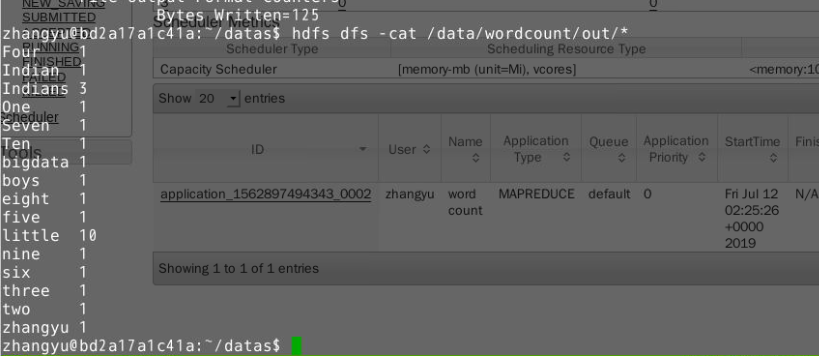
\includegraphics[width=\linewidth]{hadoop/mapred-example.png}
	
	提交运行MapReduce的WordCount例子的结果

	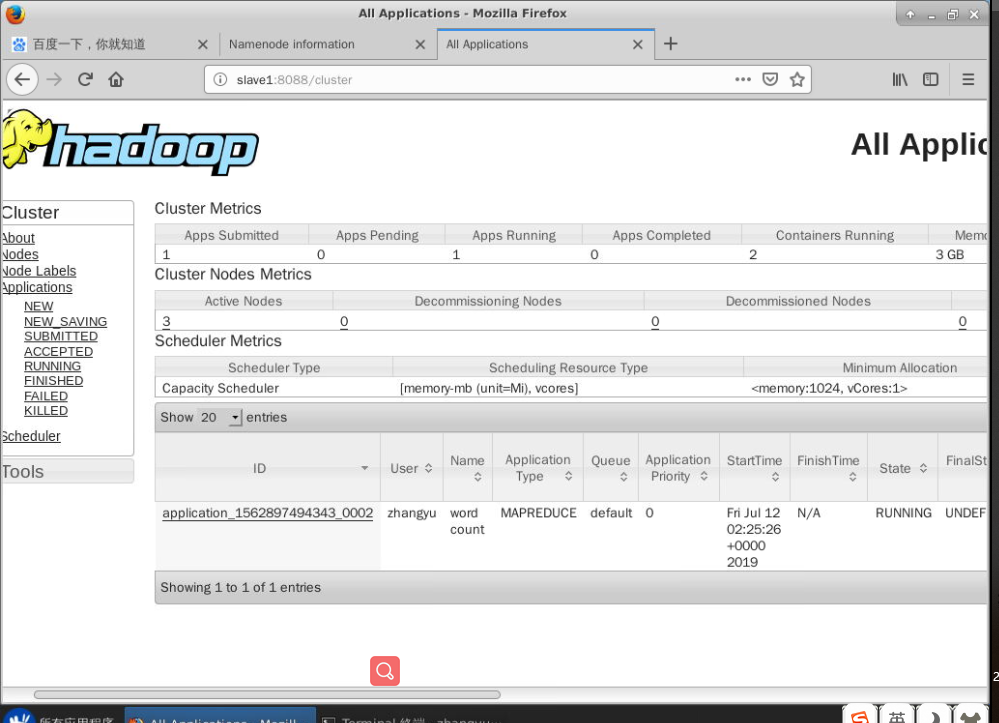
\includegraphics[width=\linewidth]{hadoop/mapreduceweb1.png}

	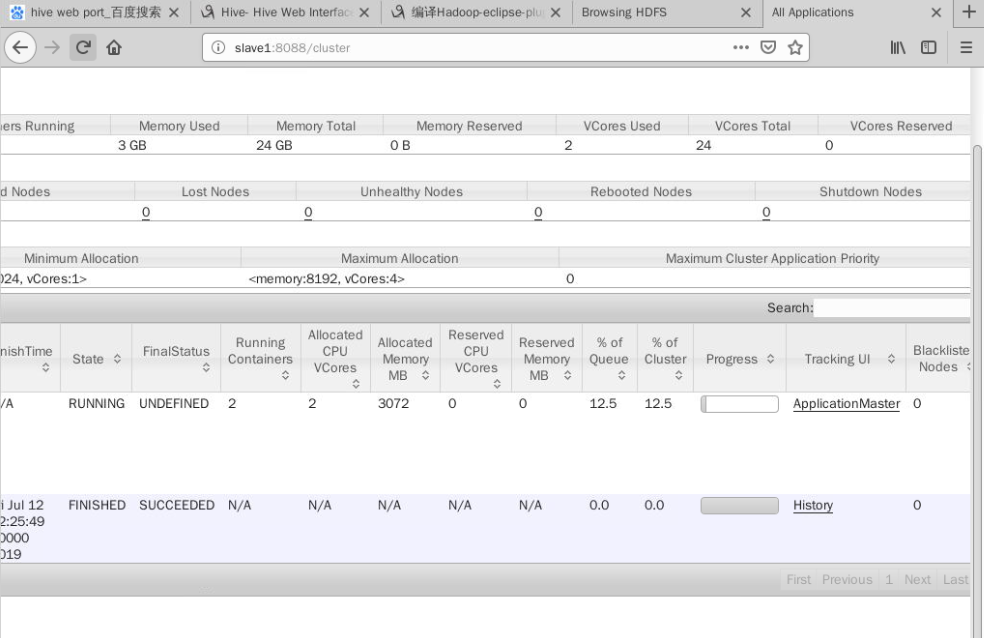
\includegraphics[width=\linewidth]{hadoop/mapreduceweb2.png}
	
	可以看到所有的提交的作业的运行情况、资源占用情况、运行还有多长时间结束等信息
\end{center}

\subsection{MapReduce编程实践}

下面以WordCount例子作为编程实例记录下来,关于MapReduce的原理,这里不做过多的讲解。

首先,在本地创建3个文件:\lstinline{file001}、\lstinline{file002}、\lstinline{file003}。

\begin{lstlisting}[style=mysh,title=file001]
Hello world
Connected world
\end{lstlisting}

\begin{lstlisting}[style=mysh,title=file002]
One world 
One dream
\end{lstlisting}

\begin{lstlisting}[style=mysh,title=file001]
Hello Hadoop 
Hello Map 
Hello Reduce
\end{lstlisting}

将上述3个文件放入\lstinline{input}文件夹中,用\lstinline{hdfs dfs -put}命令将
\lstinline{input}文件夹上传至DFS上。下面就可以开始编程了。

\begin{lstlisting}[style=myxml,title=POM依赖]
<dependency>
	<groupId>org.apache.hadoop</groupId>
	<artifactId>hadoop-common</artifactId>
	<version>3.1.2</version>
</dependency>
<dependency>
	<groupId>org.apache.hadoop</groupId>
	<artifactId>hadoop-mapreduce-client-core</artifactId>
	<version>3.1.2</version>
</dependency>
\end{lstlisting}

首先是编写Map程序:
Hadoop MapReduce框架已经在类Mapper中实现了 Map 任务的基本功能。为了实现Map任务,开发者只需要继承类Mapper,并实现该类的\lstinline{map}函数。
为实现单词计数的Map任务,首先为类Mapper设定好输入类型和输出类型。这里,Map 函数的输入是<key,value>形式,其中,key是输入文件中一行的行号,value 是该行号对应的一行内容。
所以,Map函数的输入类型为\lstinline{<IntWritable,Text>}。Map 函数的功能为完成文本分割工作,Map 函数的输出也是 <key,value> 形式,其中,key 是单词,value 为该单词出现的次数。所以,Map 函数的输出类型为\lstinline{<Text, IntWritable>}。
以下是单词计数程序的Map任务的实现代码。

\lstinputlisting[style=customjava, title=CoreMapper.java]{docs/hadoop/java/CoreMapper.java}

在上述代码中,实现 Map 任务的类为\lstinline{CoreMapper}。该类首先将需要输出的两个变量\lstinline{one}和\lstinline{label}进行初始化。

\begin{itemize}
	\item 变量\lstinline{one}的初始值直接设置为 1,表示某个单词在文本中出现过。
	\item Map 函数的前两个参数是函数的输入参数,value 为 Text 类型,是指每次读入文本的一行,key 为 Object 类型,是指输入的行数据在文本中的行号。
\end{itemize}

\lstinline{StringTokenizer}类将 value 变量中文本的一行文字进行拆分,拆分后的单词放在\lstinline{tokenizer}列表中。然后程序通过循环对每一个单词进行处理,把单词放在\lstinline{label}中,把\lstinline{one}作为单词计数。
在函数的整个执行过程中,\lstinline{one}的值一直是 1。在该实例中,key 没有被明显地使用到。context 是 Map 函数的一种输出方式,通过使用该变量,可以直接将中间结果存储在其中。

编写 MapReduce 程序的第二个任务就是编写 Reduce 程序。在单词计数任务中,Reduce 需要完成的任务就是把输入结果中的数字序列进行求和,从而得到每个单词的出现次数。

在执行完 Map 函数之后,会进入 Shuffle 阶段,在这个阶段中,MapReduce 框架会自动将 Map 阶段的输出结果进行排序和分区,然后再分发给相应的 Reduce 任务去处理。经过 Map 端 Shuffle 阶段后的结果如表 3 所示。

\lstinputlisting[style=customjava, title=CoreReducer.java]{docs/hadoop/java/CoreReducer.java}

最后是Main函数,需要在Main函数中指定Job,然后将定义的Mapper和Reducer添加到Job中。

\lstinputlisting[style=customjava, title=WordCount.java]{docs/hadoop/java/WordCount.java}

运行代码,需要将代码进行打包,然后提交到集群中才能运行。这里采用Maven Package的方法打包应用,形成Jar包后用
\lstinline{hadoop jar}命令提交。

\begin{lstlisting}[style=mysh,title=提交WordCount到集群]
# arg1 jar包名称, arg2 主类名 arg3 输入目录 arg4 输出目录
$ hadoop jar hadoopdemo-1.0.jar WordCount /input /output
\end{lstlisting}

程序运行较慢,运行之后的输出结果如下图:

\begin{figure}[h]
	\centering
	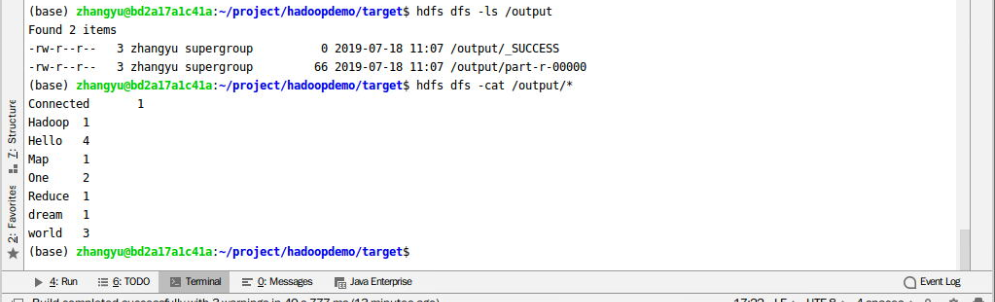
\includegraphics[width=\linewidth]{hadoop/result.png}
	\caption{提交WordCount到集群运行结果}
	\label{fig:hadoop-wordcount}
\end{figure}

